\documentclass[10pt,twocolumn,letterpaper]{article}

\usepackage{cvpr}
\usepackage{times}
\usepackage{epsfig}
\usepackage{graphicx}
\usepackage{amsmath}
\usepackage{amssymb}
\usepackage{enumitem}

\usepackage[breaklinks=true,bookmarks=false]{hyperref}

\cvprfinalcopy % *** Uncomment this line for the final submission

\def\cvprPaperID{****} % *** Enter the CVPR Paper ID here
\def\httilde{\mbox{\tt\raisebox{-.5ex}{\symbol{126}}}}

% Pages are numbered in submission mode, and unnumbered in camera-ready
%\ifcvprfinal\pagestyle{empty}\fi
\setcounter{page}{1}
\begin{document}

%%%%%%%%% TITLE
\title{Online Knowledge Distillation Methods: A Survey}

\author{Yuan Zhang\\
College of Computer Science, Zhejiang University, China\\
{\tt\small yuan\_zhang@zju.edu.cn}
% For a paper whose authors are all at the same institution,
% omit the following lines up until the closing ``}''.
% Additional authors and addresses can be added with ``\and'',
% just like the second author.
% To save space, use either the email address or home page, not both
% \and
% Second Author\\
% Institution2\\
% First line of institution2 address\\
% {\tt\small secondauthor@i2.org}
}

\maketitle
%\thispagestyle{empty}

%%%%%%%%% ABSTRACT
\begin{abstract}
Knowledge distillation is a simple but effective method to
train neural networks for meeting the low-memory and
low-latancy requirements. Offline
distillation methods utilize knowledge from
a powerful pretrained teacher, which requires
a complex two-phase training procedure.
Online methods develop an ensumble teacher to
address this problem, where networks learn from
ensumbles of themselves during the training process.
These methods are one-phase and end-to-end training scheme.
But those with high performance among
them have high memory consumption and are difficult to do
parallel training, which leaves room for improvement.
So far online methods are beyond the scope of 
distillation. They train a better network
without external knowledge from a teacher,
and give hint on exploring the maximum capacity
of a network.
\end{abstract}

%%%%%%%%% BODY TEXT
\section{Introduction}
During the last few years, deep learning has gained impressive success
in artificial intelligence. To gain better performance, the deep learning networks
is growing larger and larger. These models have achieved overwhelming
success, however the large size causes heavy computational load during inference. To
deploy such models in real-time applications or on devices with limited resources,
their size should be reduced.

Knowledge distillation~\cite{hinton2015distilling} is one of the methods to reduce
network size with acceptable accuracy drop. It is a process of extracting knowledge
from a complicated teacher network to a simple student network. According to whether teacher is updated simultaneously with student, knowledge distillation methods
are categorized into online methods and offline methods. In offline methods the teacher networks
are pre-trained and fixed, thus before distillation there is a stage to train the teacher~\cite{liu2019knowledge}~\cite{mirzadeh2020improved}~\cite{passalis2020heterogeneous}~\cite{romero2014fitnets}.
Offline methods are simple and fast if the teacher network is provided. However, when the teacher network is not presented,
offline methods begin to expose their limitations:
\begin{enumerate}
   \item Training and tuning a complex teacher network costs a lot of time and effort. And this stage may be performed several times for different tasks or trying different teacher networks.
   \item There is a gap between student and teacher, more specifically, a better teacher does not grant a better student~\cite{mirzadeh2020improved}. This makes researchers wonder whether a group of weak teachers will give better performance.
   \item It is not easy to decide the teacher framework. Usually the teacher network is just a wider version of student network. However, its size cannot be arbitrarily large. As mentioned in second point,
   a wider teacher with better performance may result in a worse student.
 \end{enumerate}

The single-stage online methods are developed to address these problems.
The earliest online methods~\cite{anil2018large}~\cite{zhang2018deep} start from a group of random networks and 
learn from each other during the distillation process. Anil \etal~\cite{anil2018large} employ their method to train
large-scale distributed neural networks and prove online knowledge distillation is a universal and powerful method
to train a simple neural network. Later such methods are developed into ensumble methods, where the student networks learn
from an ensumble of themselves~\cite{chen2020online}~\cite{guo2020online}~\cite{lan2018knowledge}. In method \textbf{ONE}~\cite{lan2018knowledge} and \textbf{CL}~\cite{song2018collaborative} a branch model is used to reduce the memory cost of too many networks.

Some methods are not in the framework of ensumble network.
Method \textbf{DCM}~\cite{yao2020knowledge} appends classifiers to hidden layers so that these layers participate the online distillation process explicitly.
Method \textbf{AFD}~\cite{chung2020feature} introduces adversarial learning into online distillation.

In this paper some of ensumble online methods are discussed.
Section ~\ref{vanilla_kd} will introduce the original form of knowledge distillation, which is the basis of online knowledge distillation.
Section ~\ref{ensubmle_model} will show most online methods follow
an ensumble framework.
Section ~\ref{review} will review these methods and discuss the challenges and opportunities in online knowledge distillation.
%-------------------------------------------------------------------------
\begin{figure*}
   \begin{center}
   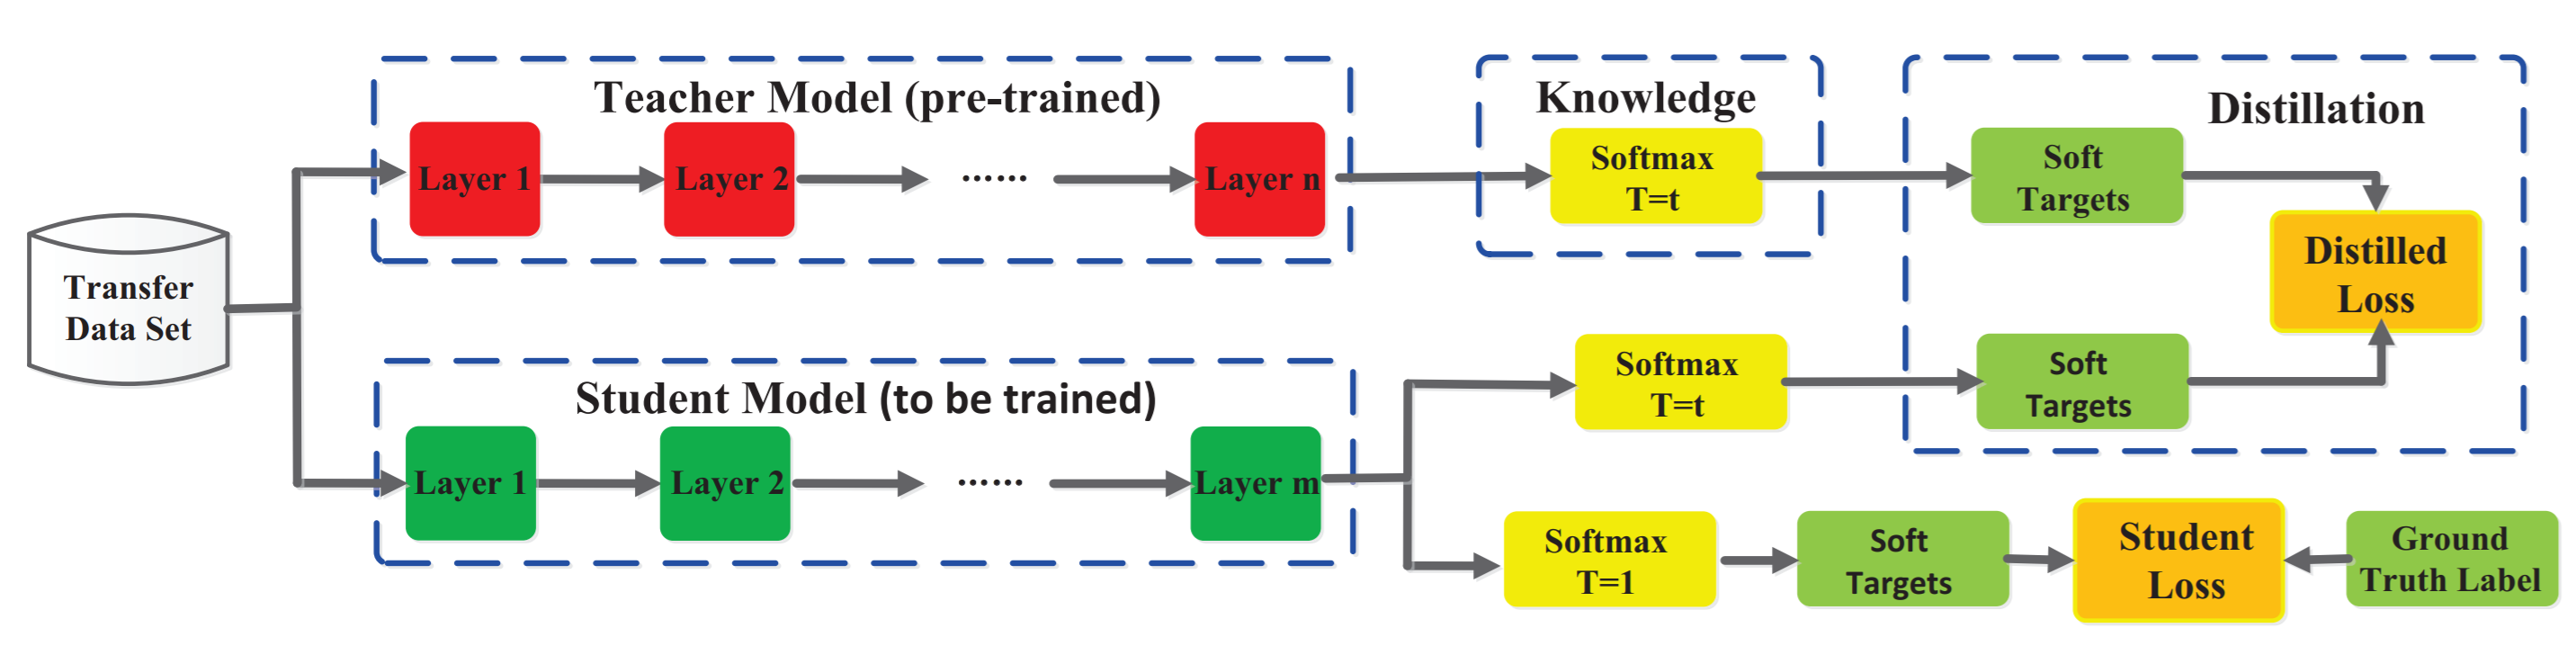
\includegraphics[width=0.9\linewidth]{vanilla_kd.png}
   \end{center}
      \caption{Vanilla knowledge distillation. Two copies of data are sent to teacher and student respectively. Then the output of teacher
is used as advice to training process of student.}
   \label{fig:vanilla_kd}
\end{figure*}
   
%------------------------------------------------------------------------
\section{Vanilla Knowledge Distillation}\label{vanilla_kd}
Figure~\ref{fig:vanilla_kd} shows the structure of vanilla knowledge distillation. Denote T as the pretrained teacher network and
denote S as the student network to be trained. Two copies of data are sent to T and S respectively.
The knowledge extracted from output of T is used to direct the training of S.

Formally, suppose there is a classification task with a labeled dataset $\mathcal D=\{(x_i, y_i)\}_i^n$, and $f_S(x;\theta):\mathcal X\mapsto\mathbb{R}^m$ is the logits function of the student network S. The parameters of T is fixed
during distillation so that function $f_T(x)$ without parameters is used to denote its logits function.

Equation~\eqref{eqn:kd_loss} gives the distillation loss, where $\textrm{H}(p, q)$ is cross entroy loss function, $\sigma$ is softmax function and $t$ is temperature of softmax function. Equation~\eqref{eqn:gt_loss} gives the
ground truth loss of classification. The final training loss is a weighted sum of this two terms.

\begin{equation}
\label{eqn:kd_loss}
   \begin{split}
   L_{\textrm{KD}}(T, S) = \sum\limits_{(x_i, y_i)\in \mathcal D}{\textrm{H}(\sigma(\frac{f_T(x_i)}{t}), \sigma(\frac{f_S(x_i; \theta)}{t}))}
   \end{split}
\end{equation}

\begin{equation}
\label{eqn:gt_loss}
L_{\textrm{GT}}=\sum\limits_{(x_i, y_i)\in \mathcal D}{\textrm{H}(\textrm{one-hot}(y_i),\sigma(f_S(x_i; \theta)))}
\end{equation}

%------------------------------------------------------------------------
\section{Ensumble Model}\label{ensubmle_model}
An ensumble model will be proposed here.
Then the text will explain how most online methods fit in this model.

Suppose a group of student networks $S_1,\dots, S_s$.
Now there is no powerful pretrained teacher networks.
A group of weighted sums of student logits becomes the teacher logits,
as calculated in Equation~\eqref{eqn:ensumble}, where
$\{w_{ij}; i, j=1,\dots,s\}$ are weights and $\Theta={\theta_1,\dots,\theta_s}$ is all student parameters. Note that these weights
can be updated, in method \textbf{ONE}~\cite{lan2018knowledge} and \textbf{OKDDip}~\cite{chen2020online}
they are a part of the network, in method \textbf{KDCL}~\cite{guo2020online} they are calculated after several iterations.

\begin{equation}
\label{eqn:ensumble}
f_{T_i}(x; \Theta) = \sum\limits_{j=1,\dots,s}{w_{ij} f_{S_j}(x; \theta_j)}
\end{equation}

Then these sums are used to teach students in the same way as Equation~\eqref{eqn:kd_loss}. The distillation loss is given by Equation~\eqref{eqn:ensumble_loss}.
\begin{equation}
\label{eqn:ensumble_loss}
L_{\textrm{ensumble}}=\sum\limits_{i=1,\dots,s}{L_{\textrm{KD}}(T_i, S_i)}
\end{equation}

Also the ground truth loss in Equation~\eqref{eqn:gt_loss} for each student is added in the final total loss. Some methods also consider
the ground truth loss for the ensumbles.

Most online methods follow the above framework. In \textbf{ONE}~\cite{lan2018knowledge}, the weights are nodes of the networks and involve the backward process.
In \textbf{OKDDip}~\cite{chen2020online} they are attentions calculated by the layer before logit layer. Method \textbf{DML}~\cite{zhang2018deep} does not strictly fit the framework, it
aggregates difference of each pair of student networks as the knowledge distillation loss. However, this loss is approximate to the loss from the above framework where each teacher is
an the average of all other student logits.

Here comes the question:
How can we get a good group of
weights? \textbf{OKDDip}~\cite{chen2020online} answers
this question with attention mechanism~\cite{vaswani2017attention}, letting neural networks learn weights automatically.
\textbf{KDCL}~\cite{guo2020online} suppose the better linear
combination of student logits gives better result,
and transform this problem to an optimization problem.
Yet there is no powerful theory or practical result to show how to get a better group of weights.


\begin{figure*}
\begin{center}
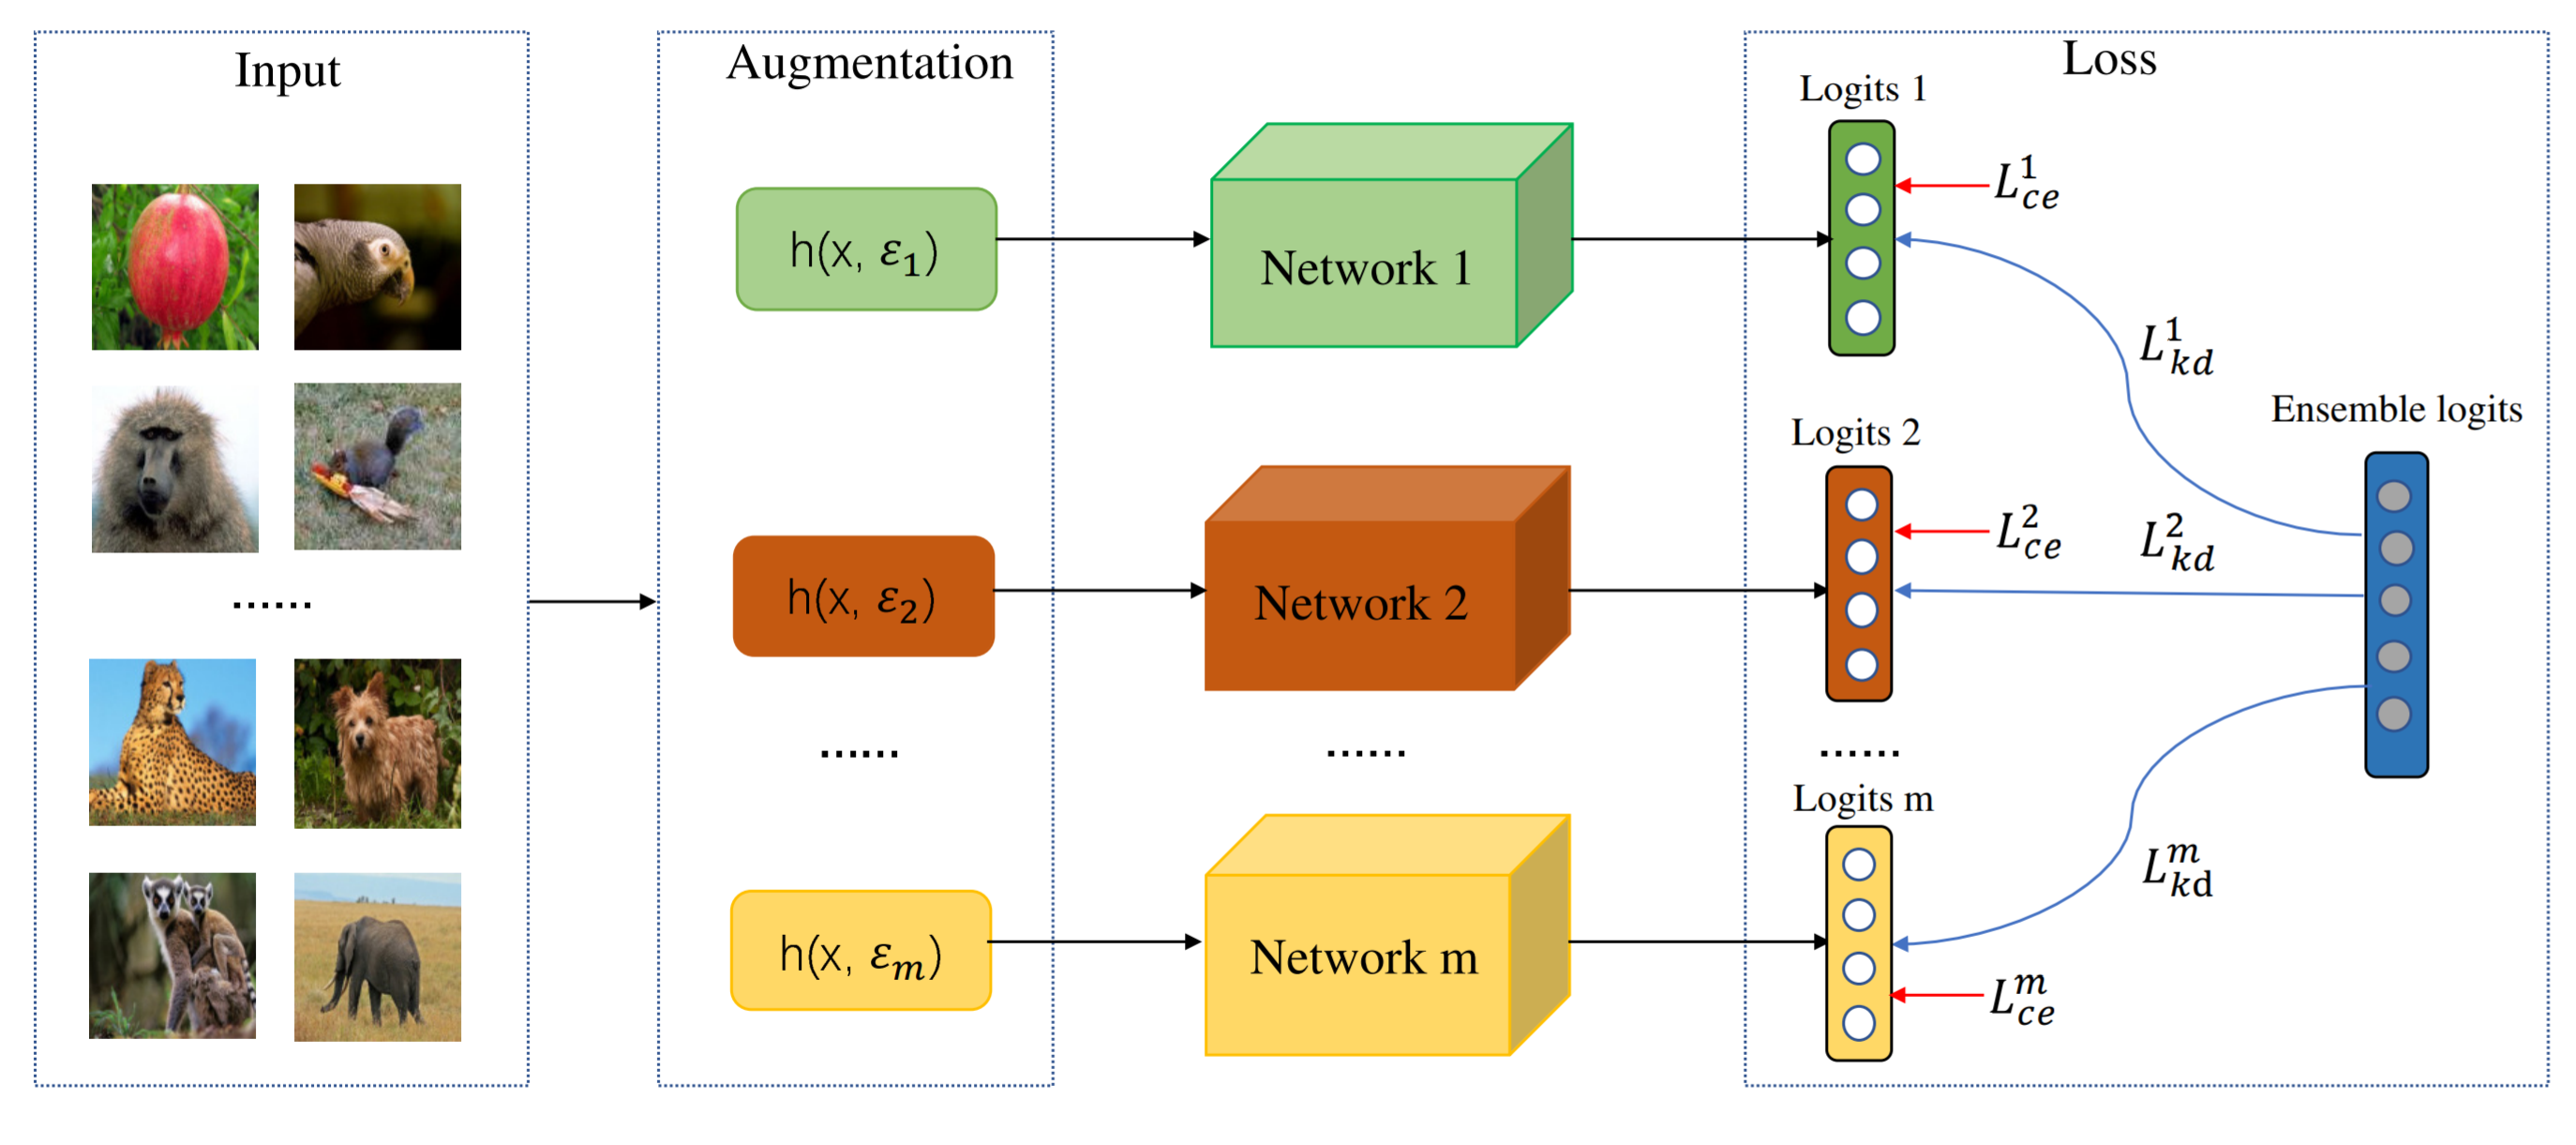
\includegraphics[width=0.9\linewidth]{ensumble_teacher.png}
\end{center}
   \caption{The teacher logits in ensumble model. Different but similar input copies are sent to different student networks. The ensumble logits come from the output of the student networks. Then they are used as the teacher output for distillation.}
\label{fig:ensumble_teacher}
\end{figure*}

%------------------------------------------------------------------------
\section{Challenges and Opportunities}\label{review}
\subsection{Utilization of Hidden Layers} Note that inner layers can be a part of the knowledge to distill.
Although more and more offline methods are utilizing knowledge from hidden layers, online methods hardly use this information.
The challenge to use inner layers is that
only same layers across networks can be ensumbled.
Offline methods use FC, CNN or attention to match layers~\cite{chen2021cross}~\cite{romero2014fitnets}~\cite{yao2020knowledge}~\cite{DBLP:journals/corr/ZagoruykoK16a}.
Online method \textbf{DCM}~\cite{yao2020knowledge} adds classifiers to hidden layers and align output size,
but this method is both time consuming and memory consuming.

\subsection{Memory Usage}
More networks give better performance~\cite{du2020agree}~\cite{wu2021peer}.
However several networks are trained
simultaneously so the number of networks is
limited by GPU memory capacity. \textbf{ONE}~\cite{lan2018knowledge}
uses a branch model to reduce memory usage in which different networks
share the same parameters at first several layers.
In method \textbf{CL}~\cite{song2018collaborative} a tree model is used. As
depicted in Figure~\ref{fig:tree_model}, all networks share parameters at root layers,
networks share parameters in groups at inner layers and networks become individual at leave layers.

Though parameter sharing is an attractive idea it reduces performance,
after all more parameters means a lot. So it would be better to explore
the field of parallel training. Anil \etal~\cite{anil2018large} has tried to
do large-scale parallel training on \textbf{DML}\cite{zhang2018deep}.
However other online methods with complicated structure are difficult to
split their calculation process, limiting their usage in real world.

\begin{figure}[t]
   \begin{center}
   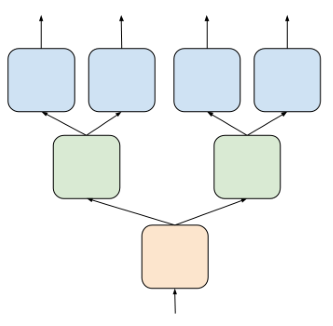
\includegraphics[width=0.6\linewidth]{hierarchical.png}
   \end{center}
      \caption{Tree Model. Split network structure into three
continuous parts. Four networks share the same parameters at first part. At second part two networks share the same parameters. And the four networks are individual at the last part.}
   \label{fig:tree_model}
\end{figure}

\subsection{Network Capacity}
Online Knowledge Distillation is more than just
a scheme of knowledge distillation.
In offline knowledge distillation provided with powerful pretrained teachers,
the students outperforms those trained directly.
This indicates that the capacity of a small network is much larger
than we can reached so far. This is also proved by \textbf{ShuffleNet}~\cite{ma2018shufflenet} and \textbf{MobileNet}~\cite{DBLP:journals/corr/HowardZCKWWAA17}.

In online methods, even the hint from teacher
is not provided, the network themselves reach
a better performance than plain training process.
Thus such methods may provide hint on reaching 
the maximum capacity of a network.
%------------------------------------------------------------------------
\section{Conclusion}
Online methods are one-phase and end-to-end
training scheme. They do not require a powerful
pretrained teacher, which is difficult to find
in variety of real world tasks.
Mainstream online methods follow
the ensumble framework proposed in Section~\ref{ensubmle_model}.
But their performance is limited by the number
of branches.
Online methods suitable for parallel computing
will perform better in real world use because 
number of branches is
hardly limited by GPU memory.
Actually, online distillation is beyond the scope of 
knowledge distillation. It becomes a scheme for
normal network training. When training a small network,
online distillation methods can be applied to
get a set of parameters with much better performance than
directly training this network.


{\small
\bibliographystyle{ieee_fullname}
\bibliography{a}
}

\end{document}
